\documentclass[border=5pt]{standalone}
\usepackage{amsmath}
\usepackage{tikz}
\usetikzlibrary{arrows.meta,positioning,fit,calc,shapes.geometric}

% Macros replicated from main.tex
\newcommand{\Problem}{SALBP-PPC}
\newcommand{\Qmax}{Q_{\max}}

\begin{document}
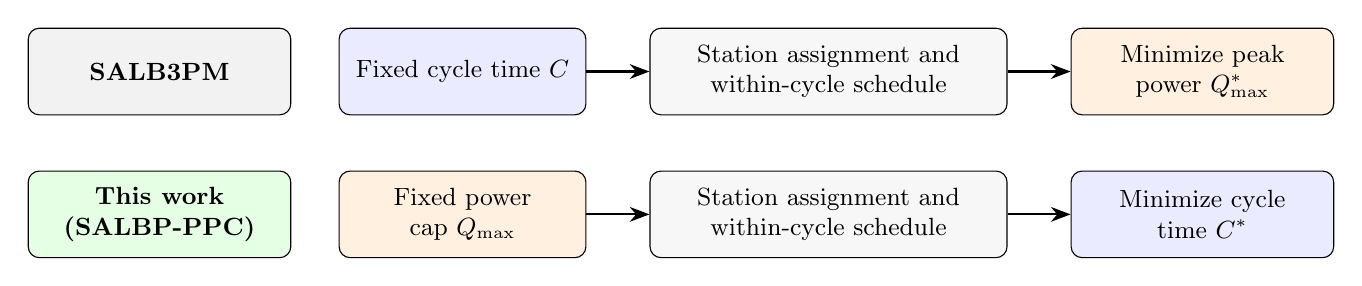
\begin{tikzpicture}[
  rowlabel/.style={draw,rounded corners,align=center,minimum height=11mm,
    text width=31mm,font=\small\bfseries},
  fixed/.style={draw,rounded corners,align=center,minimum height=11mm,
    text width=29mm,font=\small},
  model/.style={draw,rounded corners,align=center,minimum height=11mm,
    text width=43mm,font=\small},
  goal/.style={draw,rounded corners,align=center,minimum height=11mm,
    text width=31mm,font=\small},
  arr/.style={-{Stealth[length=2.5mm]},thick},
  note/.style={font=\scriptsize,align=center,text=black!70}
]
\node[rowlabel,fill=gray!10] (prior) {SALB3PM};
\node[fixed,fill=blue!8,right=6mm of prior] (fixedc) {Fixed cycle time $C$};
\node[model,fill=gray!6,right=8mm of fixedc] (modelq)
  {Station assignment and within-cycle schedule};
\node[goal,fill=orange!12,right=8mm of modelq] (minq)
  {Minimize peak\\power $Q^*_{\max}$};

\node[rowlabel,fill=green!10,below=7mm of prior] (present)
  {This work\\(\Problem)};
\node[fixed,fill=orange!12,right=6mm of present] (fixedq)
  {Fixed power cap $\Qmax$};
\node[model,fill=gray!6,right=8mm of fixedq] (modelc)
  {Station assignment and within-cycle schedule};
\node[goal,fill=blue!8,right=8mm of modelc] (minc)
  {Minimize cycle\\time $C^*$};

\draw[arr] (fixedc)--(modelq);
\draw[arr] (modelq)--(minq);
\draw[arr] (fixedq)--(modelc);
\draw[arr] (modelc)--(minc);
\end{tikzpicture}
\end{document}
